\chapter{Part 2: Prediction of Monsoon Onset}
\label{c:part2}
The onset of the ISM plays a crucial role in the daily lives of the Indian population as well as the Indian economy overall. Whether the ISM is a blessing or a curse mostly depends on the timing and the strength and durability of monsoonal rainfalls. While we have analyzed the distribution of extreme rainfall events in the previous chapter, this chapter is fully dedicated to the problem of ISM onset prediction. We focus on the monsoon onset over Kerala (MoK), as it marks the beginning of the yearly monsoon season.

Our approach to predicting



\section{The ERA-Interim Dataset}
\label{st:era_interim}
The ERA-Interim dataset is a global atmospheric reanalysis product created by the ECMWF. Reanalysis produces like ERA-Interim are created by

\begin{table}[h]
  \centering
  \begin{tabular}{rl}
    \toprule
    \textbf{ID} & \textbf{Description} \\
    \midrule
    \textbf{msl} & Mean-Sea Level Pressure \\
    \textbf{r} & Relative Humidity at 1000hPa \\
    \textbf{t} & Temperature at 1000hPa \\
    \textbf{u700} & U-Component of Wind at 700hPa \\
    \textbf{v700} & V-Component of Wind at 700hPa \\
    \textbf{u200} & U-Component of Wind at 200hPa \\
    \bottomrule
  \end{tabular}
  \caption{List of features from ERA-Interim that are used in this work.}
  \label{tab:era_features}
\end{table}

\section{Related Work}
[TODO: filler]


\subsection{Prediction of monsoon onset and variability}
\label{sst:related_prediction}
[TODO:  describe other methods that have been proposed for onset prediction (~1 page)]

\subsection{Convolutional recurrent neural networks}
\label{sst:neural_networks}
Many of our experimental models are based on a relatively new approach to training neural networks on spatiotemporal data. We specifically refer to the work of \citet{Shi.2015}, where a newly defined \textit{ConvLSTM} neural network layer was first applied to precipitation forecasting. Due to the reliance of many of our models on these layers, this section is thought to provide intuition about their inner workings. We assume that the reader is familiar with neural network principles for the remainder of this work. However, as convolutional and recurrent layers are what ConvLSTM layers are based on, we explain some of their characteristics where needed.

ConvLSTM networks as introduced by \citet{Shi.2015} were originally used for the problem of precipitation nowcasting, the primary goal of which is described as giving a ``precise and timely prediction of rainfall intensity in a local region over a relatively short period of time (e.g., 0-6 hours)'' \citep{Shi.2015}. In the aforementioned work, the authors try to predict a sequence of future precipitation radar maps from a sequence of past radar maps, essentially performing sequence-to-sequence prediction. These kinds of prediction tasks based on spatiotemporal data (where time as well as geographical location needs to be accounted for) are generally challenging, as a suitable neural network needs to be able to handle very high input and output dimensionalities.

An approach that is often used for sequence-to-sequence prediction is a two-layer architecture in which a first Long-Short Term Memory (LSTM) network reduces the input into a fixed-length sequence (``encodes'' the input into an internal representation), while a second LSTM network then predicts an output sequence using as input the fixed-length sequence (``decoding''). This encoder-decoder framework was originally described in [TODO: cite sutskever] and has been applied to many sequence-to-sequence tasks like machine translation. However, \citet{Shi.2015} have found that the regular LSTM networks used for regular sequence-to-sequence prediction are not well suited to process spatiotemporal data. While they use an encoding-decoding pattern in their models, \citet{Shi.2015} propose a new type of network layer based on regular LSTM layers that is able to better take into account the spatial dimension of input values.

The newly proposed ConvLSTM network layer combines the concept of convolutions as applied in convolutional networks with the internal structure of regular LSTM layers. In a ConvLSTM network, the states in each LSTM-cell are represented by 3D-tensors with the same spatial dimensions as the input data. Updates to any hidden state are then performed by applying convolutions to both the input values and the previous state, meaning that the new state of any location is based on the previous and current values of its immediate neighbors \citep{Shi.2015}.

Based on the previously mentioned encoding-decoding pattern and their new ConvLSTLM network layers, \citet{Shi.2015} have built several models and evaluated them on both a generated dataset with moving digits as well as on a real radar map dataset. Over both of these evaluations, the ConvLSTM architecture outperformed a fully-connected regular LSTM architecture by a significant margin. Additionally, while the countours of the precipitation predictions were found to be blurred, they still significantly outperformed the benchmark in terms of overall precision \citep{Shi.2015}.

\newpage
\section{Prediction of Monsoon Onset using Neural Networks}
\label{st:nn_implementation}
Looking to find a model capable of learning the patterns leading up to the monsoon onset, as well as predicting the onset itself, we have evaluated many different approaches to training neural networks based on spatiotemporal datasets like TRMM and ERA-Interim. Each approach had its advantages and disadvantages, many of which we only learned through trial and error and subsequently used to build an improved architecture. Over many iterations with vastly different model architectures, we have finally gotten to a model that seems to be able to learn patterns present before the monsoon onset and, based on these patterns, predict the monsoon onset with reasonable accuracy.

The first part of this section is thus focused on our certainly most important and useful result: our final working models and their evaluation. We describe their general architecture as well as the different evaluation schemes and parameters we have used. Furthermore, we evaluate how well the models have performed over the entirety our experiments and assess the prediction capabilities from different points of view (e.g., how accurately can we predict on the 15th of May, or how accurately can we predict ten days before onset).

That being said, we would probably not have gotten to our final models without having tried many other architectures beforehand, iteratively improving upon the findings of each. The remainder of this section is therefore dedicated to a brief overview over all the model architectures we have evaluated during the creation of this work (in chronological order), along with a summary of our most important findings and results during the process.

\subsection{E4: A working model based on ERA-Interim}
\label{sst:final_model}
The neural network architectures and hyperparameter tunings that we have found to work best during our experiments are based on two main ingredients: the ERA-Interim dataset with several of its features and multiple stacked convolutional recurrent layers (ConvLSTM2D). These models are all based on the latest Keras 2.0 and Tensorflow 1.4 Python libraries, which have greatly simplified our development, as even the relatively new ConvLSTM2D layer type is already implemented and usable from the core library. The remainder of this section is dedicated to a more detailed description of the way we preprocessed the ERA-Interim dataset and built our final working model architecture using the aforementioned libraries. This specific model architecture is further also referred to as \textit{E4}, the reasons of which will be explained later on.

\subsubsection{Data preprocessing}
One of the most important parts during the process of creating a neural network model (or any other machine learning model at that) is the preparation of the data that is to be used as its foundation. Without properly formatted input data, a neural network will typically not be able to learn any meaningful patterns. Over the course of our experiments, we have tried different datasets (TRMM and ERA-Interim) and, more importantly, many heterogenous input formats, of which each had its advantages and disadvantages (we go over all of these evaluated input formats in their respective sections).

The approach we use in our final model architecture (E4) is most easily explained through an example: given time series data before the monsoon onset in an arbitrary year, we extract a fixed-length sequence (for example, a sequence of 60 subsequent days). The sequence ends at a given distance before the onset (e.g., 14 days before) and starts 60 more days before that. Feeding this sequence (corresponding to a single training example) to our neural network model after training, we would like it to predict the number 14, which is comparable to a simple regression task. Intuitively, we ask our model the following question: "given the last 60 days, in how many days from today will the monsoon arrive?".

If we were to train our model only based on sequences that end 14 days before the onset, it would most certainly always predict the number 14, no matter the actual input. To train our model for different distances, we need to repeat the sequence extraction process many times per year, using a different distance to the monsoon onset in each repetition. Our most successful models are based on 30 training examples per year with distances in the range of $[1, 30]$ and a sequence length of around two months.

The actual preprocessing of the ERA-Interim dataset is only slightly more complex: instead of a simple time series, from which a sequence is extracted, we have a time series where each timestep is represented by a multidimensional matrix (a \textit{3D-tensor}). For each location in the ERA-Interim coordinate grid as well as for each feature used from ERA-Interim (e.g., temperature), these tensors contain the value of the respective feature at the respective location (at that timestep). This is more intuitively shown in \cref{fig:e4_preprocessing}.

\begin{figure}[h]
  \centering
  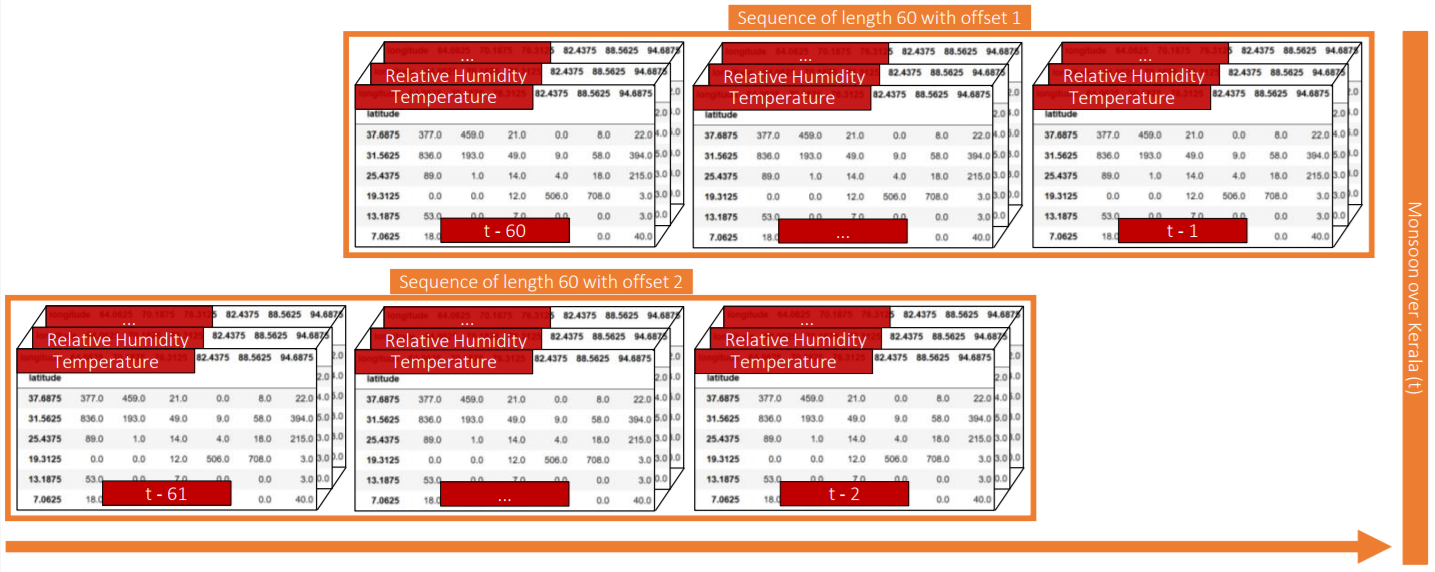
\includegraphics[width=\linewidth]{./99_appendix/img/E4_preprocessing}
  \caption{Data preprocessing for models of the E4 class.}
  \label{fig:e4_preprocessing}
\end{figure}

\paragraph{Normalization} An additional step during data preprocessing is often the normalization of data into certain consistent ranges. Even though neural networks could learn without normalization, it often improves and speeds up their learning process. If different input features do not adhere to the same distribution (e.g., temperature and rainfall), the different magnitudes can lead to problems during the optimization process (when multiplying with the learning rate). When processing the ERA-Interim dataset into a training, validation and test set, we therefore apply statistical standardization to center the mean of each feature separately. To prevent the introduction of any bias, the mean and standard deviation of the training set are reused when normalizing the validation and test sets.

\clearpage
\subsubsection{Model architecture}
It is not hard to see that a single ERA-Interim coordinate grid is inherently similar to a simple multichannel image: we have a height (latitudes), a width (longitudes) and multiple channels (e.g., temperature and relative humidity). When working with images, convolutional neural networks are by far the most prevalent approach. They have led to great progress in image recognition and other domains. However, 2D-convolutions are not directly applicable to multiple images ordered in a sequence (like a movie). Instead, they first need to be combined with recurrent network structures like LSTM.

We have already introduced a recent approach to the problem of learning from spatiotemporal data: the ConvLSTM2D neural network layer (\cref{ssst:conv_lstm_2d}). In our case, this layer performed much better than a simple stacking of convolutional and recurrent layers, making it the most important part of many of our models (including E4). With ConvLSTM2D at its core, the E4 model architecture performs a regression by flattening the final output of the ConvLSTM2D layers and passing it through multiple dense layers, the final one of which has only a single neuron (and thus yields a single number). As an optional addition, time-distributed convolutional and pooling layers can be applied before passing the sequence into the ConvLSTM2D layers, adding further feature detection and dimensionality reduction capabilities. An exemplary model based on the described architecture is shown in \cref{fig:e4_architecture}.

\begin{figure}[h]
  \centering
  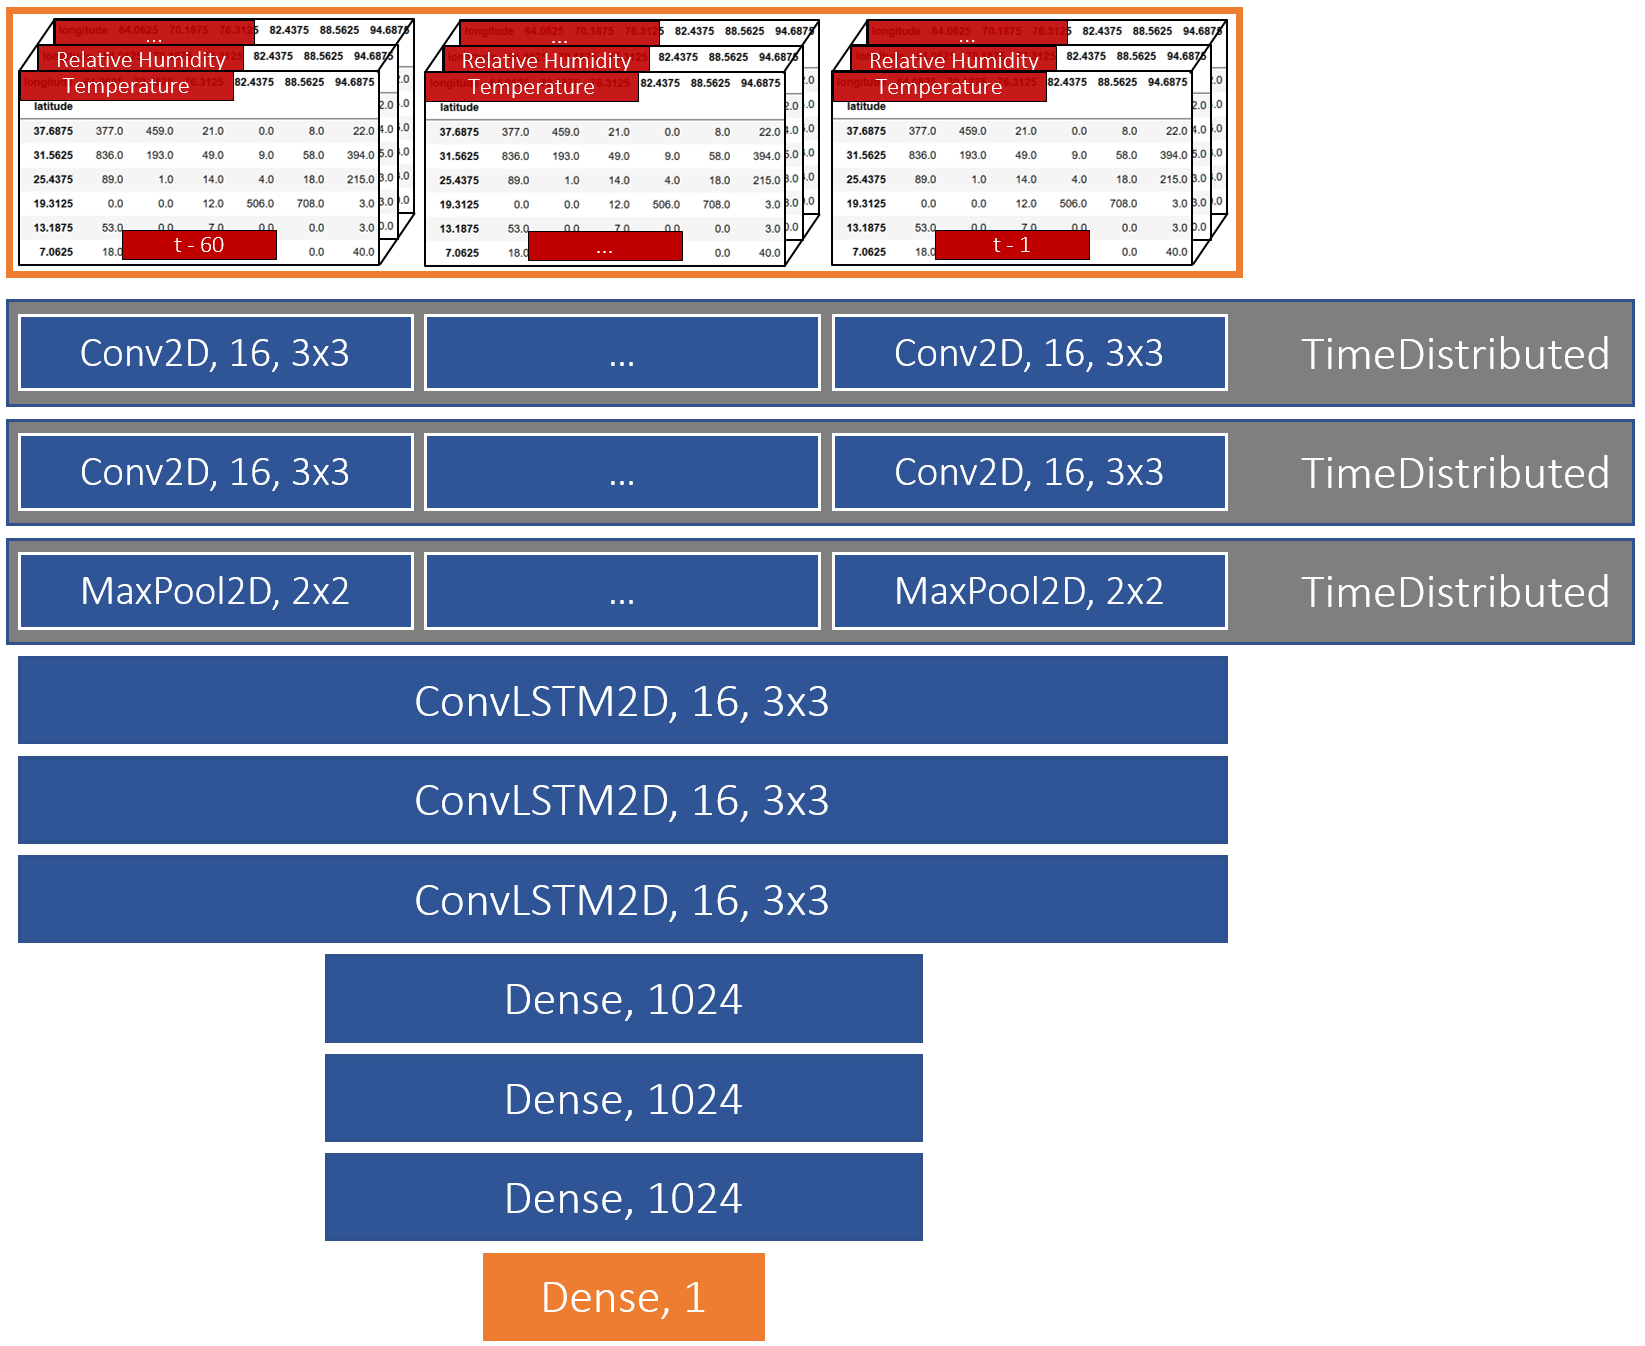
\includegraphics[width=0.8\linewidth]{./99_appendix/img/E4_architecture}
  \caption{Exemplary model architecture of the E4 class.}
  \label{fig:e4_architecture}
\end{figure}

\paragraph{Regularization} To reduce the tendency of the model to overfit to the training set, we apply L2-regularization to the kernels of all types of layers (Conv2D, ConvLSTM2D, Dense). This increases the loss whenever the model's internal representation of the problem gets too complex, effectively improving its ability to generalize. Also, we can and do most often use dropout after each layer. However, the exact regularization and dropout parameters vary with each tuning.

\paragraph{Batch normalization} To speed up the training of our models, we make use of batch normalization after each layer in the models. During the training process, a batch normalization layer normalizes (``centers'') the activations of each batch of training examples, preventing even small initial shifts in batch statistics (``internal covariate shift'') to grow increasingly large when processed by many subsequent layers in a deep network.

\subsubsection{Model evaluation}
On our search for the best configuration to train our models with, we have performed 45 experiments for this final model architecture alone. The parameter space we were searching through can be split into two major categories: ``hyperparameters'', referring to the parameters that are typically heavily tuned to improve model performance (e.g., learning rate, dropout rates, kernel sizes, etc.), and a second category that is more fundamental, as it already influences the data when it is being preprocessed. The choice of datasets and features thereof, as well as the amount of data that is being fed to the model (e.g., the sequence length), are exemplary parameters that we assign to the latter category. An overview of such ``meta-hyperparameters'' is shown in \cref{tab:meta_parameters}.

\begin{table}[h]
  \centering
  \begin{tabular}{|r|c|c|c|c|c|c|}
    \hline
    \textbf{ERA-Features} & \multicolumn{1}{c|}{msl/r/t} & \multicolumn{2}{c|}{msl/r/t/u700/v700} & \multicolumn{3}{c|}{msl/r/t/u700/v700/u200} \\
    \hline
    \textbf{Onset Dates} & \multicolumn{3}{c|}{IMD (1979-2017)} & \multicolumn{3}{c|}{Objective (1979-2007) + IMD (2007-2017)} \\
    \hline
    \textbf{Sequence Length} & 32 & 42 & 47 & 62 & 77 & 92 \\
    \hline
    \textbf{Sequence Offset} & 0-8 & 0-21 & 0-22 & 5-25 & 0-30 & 1-30 \\
    \hline
  \end{tabular}
  \caption{``Meta-hyperparameters'' as they have been used in the final E4-class models. IMD onset dates until 2007 are extracted from \citet{Singh.2009} and concatenated with official IMD dates (2007-2017). Objective onset dates are extracted from the same source, but then also concatenated with IMD dates. The Sequence Offset specifies the range of offsets that is generated (meaning that for a value of 1-30, 30 examples are generated for each year). Details about the ERA-Features can be found in \cref{tab:era_features}. }
  \label{tab:meta_parameters}
\end{table}

\paragraph{Training, validation and test set}
The ERA-Interim dataset was split into three fixed sets for each of our experiments: a training, validation and test set. As can be seen in \cref{tab:train_test_split}, we originally started with only three years in the validation and five years in the test set (out of 38 years). When many models seemed to fit to the training set very well, we decided to reduce the size of the training set, extending both the validation and test set (to four and eight years, respectively).

Because the ``objective'' onset dates stem from two different distributions (data that follows the objective definition is available until 2007, after which the dates come from the IMD), model performance was much worse when using the second split. After it was reduced to the years 1979-2005, the training set did no longer contain years based on the official IMD dates, while most of the validation and test set were based on these IMD dates. Unsurprisingly, the overall strongest overfitting was observed in the few experiments that were carried out this way. As a remedy to this problem, we devised a third split scheme with a more appropriate distribution of years, which was then used successfully for the remainder of the experiments.

It needs to be noted that tuning models on one split scheme and changing this scheme afterward could introduce bias, as years that the model might have trained on in a previous experiment could suddenly belong to the test set. It cannot be completely disqualified that some bias might be present in our later models due to these changes, even though we took care to introduce the least possible of it. It is typically best to devise one split scheme and apply this scheme to all experiments.

\begin{table}[h]
  \centering
  \begin{tabular}{rccc}
    \toprule
    & \textbf{Split 1} & \textbf{Split 2} & \textbf{Split 3} \\
    \midrule
    \textbf{Validation} & 2010-2012 & 2006-2009 & 80/90/00/10/16 \\
    \textbf{Test} & 2013-2017 & 2010-2017 & 85/95/03/04/05/14/15/17 \\
    \midrule
    \textbf{Experiments} & 0-27 & 28-31 & 32-45 \\
    \bottomrule
  \end{tabular}
  \caption{The three different splits that have been applied to the dataset in the experiments for E4.}
  \label{tab:train_test_split}
\end{table}

\paragraph{Evaluation schemes}
Over the course of our experiments, we have used various combinations of the previously described ``meta-hyperparameters'', leading to what can be called \textit{evaluation schemes}. An evaluation scheme is a group of experiments that are based on the same high-level parameters but have been tuned using different hyperparameters. We can reduce the total of our 45 experiments to 17 such evaluation schemes, each consisting of up to nine experiments. The listing in \cref{tab:evaluation_schemes} shows these 17 evaluation schemes along with their configuration. For each evaluation scheme, we therein show the features from ERA-Interim that its experiments were based on, the source of onset datasets used, the number of days in an input sequence, as well as the number of training examples per year and the minimum offset of these training examples.

\begin{table}[h]
  \centering
  \begin{tabular}{cccccc}
    \toprule
    \textbf{ID} & \textbf{ERA-Features} & \textbf{Onset Dates} & \textbf{Seq. Length} & \textbf{Seq. Offset}  & \textbf{\#} \\
    \midrule
    EV01 & msl/r/t & IMD & 47 & 1/30 & 1 \\
    EV02 & msl/r/t & IMD & 62 & 1/30 & 2 \\
    EV03 & msl/r/t & IMD & 77 & 1/30 & 1 \\
    EV04 & msl/r/t & Objective+IMD & 62 & 5/25 & 3 \\
    EV05 & msl/r/t & Objective+IMD & 62 & 0/30 & 3 \\
    EV06 & msl/r/t & Objective+IMD & 62 & 1/30 & 3 \\
    EV07 & msl/r/t/u700/v700 & IMD & 62 & 1/30 & 9 \\
    EV08 & msl/r/t/u700/v700 & Objective+IMD & 32 & 0/30 & 1 \\
    EV09 & msl/r/t/u700/v700 & Objective+IMD & 62 & 0/21 & 3 \\
    EV10 & msl/r/t/u700/v700 & Objective+IMD & 62 & 0/22 & 8 \\
    EV11 & msl/r/t/u700/v700 & Objective+IMD & 62 & 0/30 & 3 \\
    EV12 & msl/r/t/u700/v700 & Objective+IMD & 62 & 1/30 & 2 \\
    EV13 & msl/r/t/u700/v700 & Objective+IMD & 62 & 0/8 & 3 \\
    EV14 & msl/r/t/u700/v700 & Objective+IMD & 92 & 0/30 & 1 \\
    EV15 & msl/r/t/u700/v700/u200 & Objective+IMD & 42 & 0/30 & 1 \\
    EV16 & msl/r/t/u700/v700/u200 & Objective+IMD & 62 & 0/30 & 1 \\
    \midrule
    \multicolumn{5}{r}{\textbf{Total number of experiments}} & 45 \\
    \bottomrule
  \end{tabular}
  \caption{Evaluation schemes for the E4-class models and the corresponding number of experiments, based on the ``meta-hyperparameters'' as shown in \cref{tab:meta_parameters}. Details about the ERA-features can be found in \cref{tab:era_features}}
  \label{tab:evaluation_schemes}
\end{table}

\paragraph{Experimental conditions}
The experiments were run in different environments and are explicitly marked as such: either on a local GPU, the Kraken cluster or a Paperspace\footnote{https://www.paperspace.com/} virtual machine. \cref{tab:experimental_environments} provides a more detailed overview of the environments used during the experimental phase. While all of the experiments for the E4-class of models were run on the \textit{PS} environment due to performance constraints, most earlier experiments were run locally or on Kraken.

\begin{table}[h]
  \centering
  \begin{tabular}{ ccc }
    \toprule
    \textbf{Environment} & \textbf{Trained on} & \textbf{Available memory} \\
    \midrule
    Kraken & CPU (24-cores) & 128GB RAM \\
    Local & GPU (GTX 970) & 32GB RAM, 4GB GPU \\
    Paperspace & GPU (Quadro P5000) & 30GB RAM, 16GB GPU \\
    \bottomrule
  \end{tabular}
  \caption{Runtime environments for the deep learning experiments.}
\label{tab:experimental_environments}
\end{table}

\clearpage
\subsubsection{Intermediary evaluation results}
To provide a better overview of the outcome of our experiments, we reduce the results presented to only the best experiment of any given evaluation scheme (i.e., its best performing ``hyperparameter tuning''). \cref{tab:evaluation_scheme_results} shows the loss and validation loss after some key epochs as well as after the overall final epoch. Notice that loss and validation loss measures are based on the mean-squared error (MSE) but tend to be higher due to the regularization that is additionally applied.

\begin{table}[h]
  \centering
  \begin{tabular}{crrrrrrrrrrr}
    \toprule
    \textbf{Epoch} & \multicolumn{2}{c}{\textbf{10}} & \multicolumn{2}{c}{\textbf{30}} & \multicolumn{2}{c}{\textbf{50}} & \multicolumn{2}{c}{\textbf{100}} & \multicolumn{3}{c}{\textbf{Final}} \\
    & \textbf{L} & \textbf{VL} & \textbf{L} & \textbf{VL} & \textbf{L} & \textbf{VL} & \textbf{L} & \textbf{VL} & \textbf{L} & \textbf{VL} & \textbf{\#} \\
    \midrule
    \textbf{EV01} & 48 & 132 & 37 & 85 & 30 & 87 & 15 & 72 & 11 & 68 & 500 \\
    \textbf{EV02} & 43 & 92 & 33 & 70 & 25 & 73 & 13 & 57 & 6 & 63 & 500 \\
    \textbf{EV03} & 54 & 76 & 35 & 63 & 24 & 87 & 14 & 96 & 6 & 69 & 500 \\
    \textbf{EV04} & 43 & 73 & 32 & 40 & 24 & 36 & 13 & 56 & 6 & 17 & 500 \\
    \textbf{EV05} & 69 & 86 & 41 & 54 & 25 & 45 & 17 & 26 & 12 & 24 & 500 \\
    \textbf{EV06} & 41 & 59 & 32 & 58 & 24 & 58 & 14 & 35 & 5 & 33 & 500 \\
    \textbf{EV07} & 72 & 125    &    52 & 92    &    39 & 66 &    18 & 52 & 10 & 38 & 500 \\
    \textbf{EV08} & 82 & 225    &    50 & 137 & 27 & 112    &    13 & 73 & 7 & 66 & 500 \\
    \textbf{EV09} & 41 & 38 & 41 & 39 & 40 & 37 & 39 & 38 & 38 & 37 & 227 \\
    \textbf{EV10} & 63 & 76 & 37 & 38 & 20 & 46 & 9 & 16 & 7 & 20 & 150 \\
    \textbf{EV11} & 61 & 65 & 37 & 63 & 23 & 30 & 19 & 49 & 19 & 26 & 300 \\
    \textbf{EV12} & 56 & 105    &    41 & 99    &    27 & 80    &    18 & 44 & 10 & 49 & 500 \\
    \textbf{EV13} & 6 & 10    &    7 & 5    &    7 & 5    &    6 & 5 & 6 & 5 & 117 \\
    \textbf{EV14} & 199 & 246 & 95 & 141 & 103 & 212 & 87 & 77 & 90 & 898 & 134 \\
    \textbf{EV15} & 196 & 263 & 92 & 137    &    38 & 77    &    23 & 58 & 14 & 61 & 300 \\
    \textbf{EV16} & 124 & 139 & 84 & 268    &    53 & 194 & 31 & 147 & 9 & 144 & 300 \\
    \bottomrule
  \end{tabular}
  \caption{Loss (L) and validation loss (VL) after a given number of epochs for the best experiment of each evaluation scheme. The best experiment is therein defined as whichever experiment has the lowest validation loss after its final epoch. It has to be taken into account that the range the offset can take on strongly influences the magnitude of the losses: in EV13, we had only 8 training examples per year, meaning that predictions should lie between 0 and 7 (a validation loss of 5 is thus very bad).}
  \label{tab:evaluation_scheme_results}
\end{table}

We can see that, for most of the evaluation schemes, the models were able to appropriately fit to the training set. What greatly varies is the generalization capabilities of the different model architectures, which is typical when experimenting with neural networks. We would further expect the final training losses to be even lower if regularization was omitted, which would, however, most certainly come at the cost of worse generalization.

During these 45 experiments, we have not applied any automated early stopping procedures. Such procedures are often used to interrupt the training process once the performance stops improving (or once the difference between loss and validation loss increases again). Some experiments have, however, been interrupted manually, once it became clear that their performance would most certainly only get worse (specifically EV09, EV13, and EV14).

\subsubsection{Final evaluation}
After the completion of the primary tuning phase and finding some model configurations that seemed to perform well, we wanted to reduce the variance in the test results. We thus performed a further round of evaluation where we retrained the best-performing models several times each and averaged their predictions. More specifically, we chose the five experiments that had the lowest validation loss (out of the experiments that used Split 3). These five experiments belonged to the EV02, EV06, EV07 and EV12 evaluation schemes, of which both experiments in EV02 were amongst the top five.

\paragraph{Evaluation procedure}
The final evaluations were performed as follows: first, the validation set was recombined with the training set, as it was no longer needed for tuning. This step allowed the final models to train on more data, potentially resulting in more representative results. The fixed validation set was instead replaced with a random 20\% holdout set during training (changing every epoch). The five final model configurations were then trained five times each. After the successful completion of all training rounds (consisting of 25 experiments), the predictions of repetitious experiments were averaged, yielding a final set of predictions. We hereafter refer to the final sets of experiments as 0-EV12, 1-EV07, 2-EV02, 3-EV02, and 4-EV06, corresponding to a unique identifier as well as the evaluation scheme they belong to.

\paragraph{Early stopping}
Contrary to the previous experiments, we applied early stopping with a patience of 130 epochs, meaning that if the validation loss did not decrease during more than 130 epochs, the training process was interrupted and the models immediately evaluated. Most experiments were stopped after around 200-300 epochs, while they could have run up to a full 500 epochs.

\paragraph{Test accuracy with respect to the distance from onset}
Looking at the averaged predictions of each set of experiments as shown in \cref{fig:e4_prediction_accuracy_offset}, we can see that the models trained on IMD onset dates are capable of predicting monsoon onset with quite a bit less than four days of mean-absolute error (MAE). Contrary to our previous beliefs that the objectively calculated onset dates would better represent the underlying patterns, the models based on these dates seem to perform much worse: their accuracy mostly ranges between 4-4.5 days MAE. This is partly caused by the fact that from 2007 onwards, the objective onset dates needed to be completed using official IMD dates. As such, test years after 2007 are always evaluated on official IMD dates, while the model has mostly trained on objectively calculated dates.

A further interesting pattern that can be observed is that the models seem to predict more accurately (down to 2.5 days MAE) when predictions are made close to the monsoon onset, which makes intuitive sense. However, the predictions also seem to be more accurate in all models when predictions are made more than about three weeks before the onset. There might be predictive patterns present that tend to lead the monsoon onset by several weeks.

The first model from EV02 (2-EV02) seems to perform best overall, with a short-term accuracy of about 2.5 days MAE, a mid-term accuracy of 3-3.5 days MAE and a longer-term accuracy (up to one month before the onset) of around 2.5-3 days MAE. This is, by a fair margin, below the four days MAE that was described as the error of IMD predictions. Interestingly, this model is the only model that does not use additional convolutional layers and passes the inputs directly through ConvLSTM2D (after pooling), which might mean that these additional feature detectors are not as useful as they were thought to be.

\begin{figure}[h!]
  \centering
  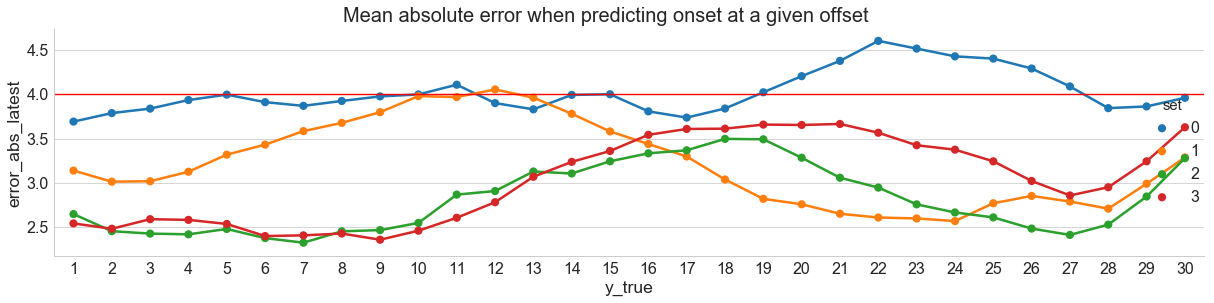
\includegraphics[width=\linewidth]{./99_appendix/img/prediction_accuracy_offset}
  \caption{The prediction accuracy of our final sets of experiments at a distance of 1-30 days from the true onset.}
  \label{fig:e4_prediction_accuracy_offset}
\end{figure}

\paragraph{Test accuracy for each test year}
A further interesting metric is the accuracy of the models when compared in-between years of the test set. Looking at the distributions in \cref{fig:e4_prediction_years}, we can see that there seem to be some years that are ``easier to predict'' than others. However, each set of models seems to display its best prediction skills in slightly different years. The year 2015 especially stands out, as the mean over all sets of models (even the two objectively trained ones) is very similar. Further analysis of the accuracy on the test years can be found in \cref{apx:prediction_ci}, where we show the accuracy of each set of models subject to a 95\% confidence interval.

\begin{figure}[h!]
  \centering
  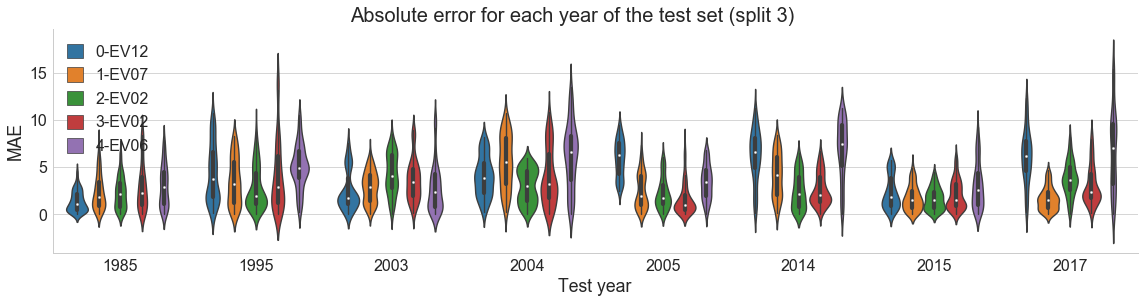
\includegraphics[width=\linewidth]{./99_appendix/img/prediction_years}
  \caption{The prediction accuracy of our final sets of experiments for the different years in the test set (1985, 1995, 2003, 2004, 2005, 2014, 2015, 2017).}
  \label{fig:e4_prediction_years}
\end{figure}

\paragraph{Test accuracy with respect to the prediction date}
The results as presented in \cref{fig:e4_prediction_accuracy_offset} can be transformed in an interesting fashion: for each prediction made on the test set, we can assign the date the prediction would have been made according to the true onset date of the corresponding year. For example, given a prediction with a true distance of five days for the year 2017 (where the onset was on the 30th of May), we would end up with the 25th of May as a prediction date. Plotting these transformed results as shown in \cref{fig:e4_prediction_accuracy_dates} allows us to see how accurate we can expect a prediction to be on any given day.

\begin{figure}[h!]
  \centering
  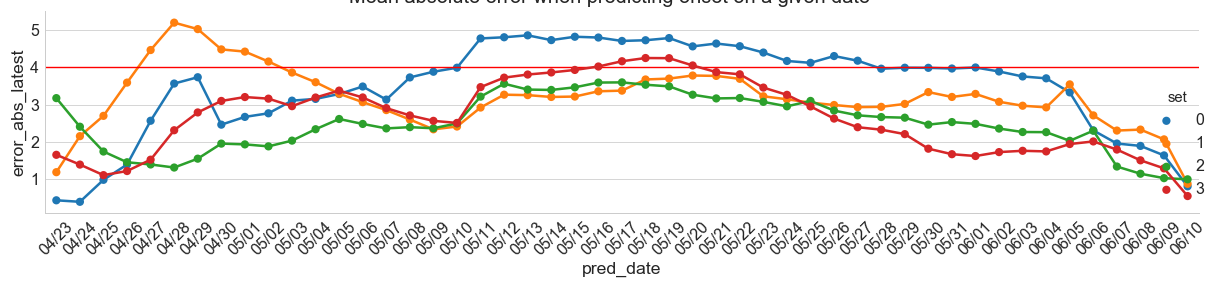
\includegraphics[width=\linewidth]{./99_appendix/img/prediction_accuracy_dates}
  \caption{The prediction accuracy of our final sets of experiments at any given date before the true onset.}
  \label{fig:e4_prediction_accuracy_dates}
\end{figure}

It is obviously much more useful to predict the onset earlier rather than later. According to \cref{fig:e4_prediction_accuracy_dates}, we might think that we would get our best predictions if we predicted towards the end of April. However, it has to be taken into account that not all dates in this visualization consist of the same number of predictions, leading to less significance of the average towards the extremes (\cref{fig:e4_prediction_dist}). As such, predictions performed around or after the 8th of May would most certainly lead to more accurate results. The prediction task could also be repeated every day after that, as our model is in its capabilities not restricted to only short- or long-term predictions.

\begin{figure}[h!]
  \centering
  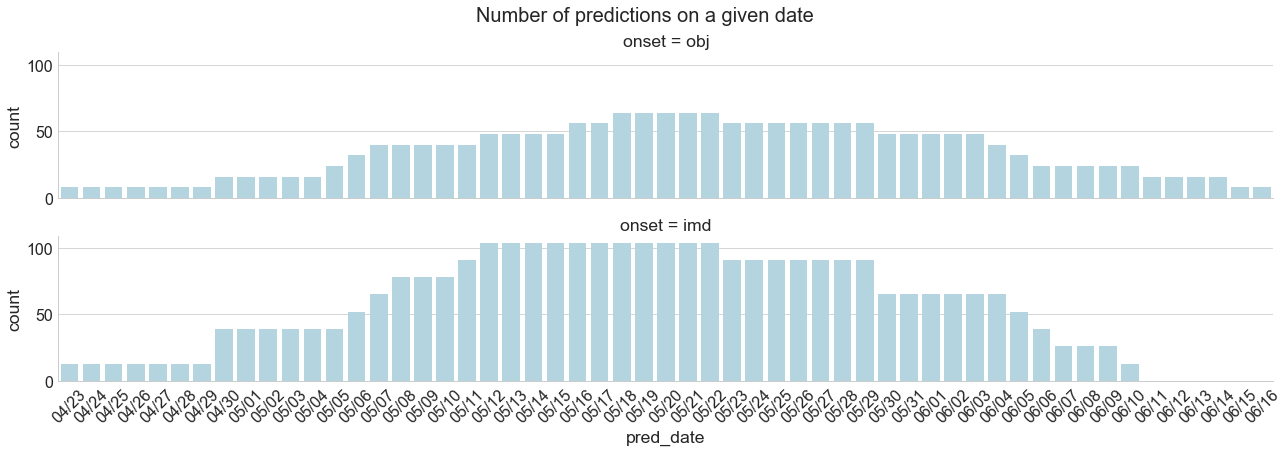
\includegraphics[width=\linewidth]{./99_appendix/img/prediction_accuracy_dates_dist}
  \caption{Number of predictions on the test set for any given prediction date.}
  \label{fig:e4_prediction_dist}
\end{figure}

\paragraph{Overall average accuracy}
When we combine the separate measures shown previously, we get a single accuracy measure over the entire test set. As shown in \cref{tab:overall_average}, 2-EV02 is the overall most accurate model, achieving an accuracy of around 2.8 days MAE. The other two models that are also based on IMD onset dates follow the first model closely, while the models based on objective onset dates are significantly lagging behind. However, this might look different if objective onset dates were available for the entirety of the training and test years (i.e., 1979-2017).

\begin{table}[h!]
  \centering
  \begin{tabular}{rccccc}
    \toprule
    \textbf{Final evaluation set} & \textbf{0} & \textbf{1} & \textbf{2} & \textbf{3} & \textbf{4} \\
    \midrule
    \textbf{Evaluation scheme} & EV12 & EV7 & EV02 & EV02 & EV06 \\
    \textbf{Onset dates} & Objective & IMD & IMD & IMD & Objective \\
    \midrule
    \textbf{Mean-absolute error} & 4.11 & 3.05 & 2.82 & 3.03 & 4.25 \\
    \bottomrule
  \end{tabular}
  \caption{Overall mean-absolute error for the five final models.}
  \label{tab:overall_average}
\end{table}

\subsection{T1-T5 and E1-E3: Other model architectures}
On the path towards the well-working E4-class of models, there were many other approaches that disappointed with their learning capabilities. However, even though they did not end up to be a working model, each model architecture we have evaluated and subsequently discarded has led to important findings, without which we could not have created a working model at all. In this section, we walk through these different variations of neural network models and shortly summarize the key takeaways of each variation.

The model variations we have evaluated differ in their network structure, in the data and features used to train the models or simply in the tuning of hyperparameters applied. \cref{tab:nn_overall_summary} summarizes the key characteristics of the models we have built and evaluated and shows how the E4-class has come to be. Each model architecture is assigned a unique version identifier that we use when referring to the specific architecture (like we already did with \textit{E4}). The identifiers are based on the type of dataset used to train the model and the variation of the model architecture used (e.g., \textit{T1}: TRMM v1, \textit{E3}: ERA-Interim v3). All of the models presented were built and trained using the latest Keras 2.0 and Tensorflow 1.3/1.4 libraries for Python.

\begin{table}[h]
  \begin{tabularx}{\linewidth}{c|X}
    \toprule
    \textbf{Model} & \textbf{Architectural Key Points} \\
    \midrule
    T1 & First trials with LSTM and TRMM; No experiments; Discarded \\
    T2 & Each location of each year as a separate example; Sequences of values for single grid cells processed with LSTM; Categorical prediction on the 11th of May (predicted MoK in 1-40 days) \\
    T3 & Each year as a separate example; One sequence of TRMM grids (daily values) per year processed with ConvLSTM2D; Numerical prediction on the 11th of May (predicted MoK in x days) \\
    T4 & Regularization for dense, convolutional and recurrent layers; Based on T3 \\
    T5 & Objective or IMD onset dates from \citet{Singh.2009}; Prediction on the 22nd of May; Based on E2 \\
    \midrule
    E1 & Training on the ERA-Interim dataset and multiple features (temperature, relative humidity); Based on T4 \\
    E2 & Objective or IMD onset dates from \citet{Singh.2009}; Prediction on the 22nd of May; Based on E1 \\
    E3 & Improved structuring of Python classes; Extraction of core model logic into base classes; Same functionality as E2; No experiments \\
    E4 & Multiple examples per year with variable offset to the onset date; Choice of additional input features; Possibility for additional 2D-convolutions before ConvLSTM2D; Switch to the functional Keras API; Based on E3 \\
    \bottomrule
  \end{tabularx}
  \caption{Overview of all neural network models that have been built \& evaluated}
  \label{tab:nn_overall_summary}
\end{table}

\subsubsection{T2: Naive classification models using TRMM}
\label{sst:nn_t2}
The first models we evaluated were classification networks based on the TRMM dataset (see \cref{st:trmm_dataset}) at various spatial resolutions (ranging from a 0.25\degree x 0.25\degree resolution to an aggregated 2.5\degree x 2.5\degree resolution).

\paragraph{Data preprocessing}
\label{ssst:nn_t2_data}
A single TRMM cell (i.e., a single location on the grid) was taken at a time and transformed into a time series for that specific location (from the first of May up to the prediction date). The latitude and longitude indices were appended in front of the time series to allow the network to learn the spatial features of each example. This led to training examples each consisting of a one-dimensional fixed-length sequence containing coordinates and daily rainfall amounts as well as a label corresponding to its category. \cref{tab:nn_t2_data} provides an overview of the structure of the examples used to train and evaluate the model.

The labels were represented as one-hot encoded vectors like $\left[ 0, ..., 1, ..., 0 \right]$. They were calculated based on the difference in days between the fixed prediction date and the monsoon onset date over Kerala. As the earliest onset in the used source \citep{Ordonez.2016} for the relevant period (1998-2017) was found to be on the 12th of May, the prediction date was set to be the 11th of May. With the latest historical onset during the available period (1887-2017) being on the 15th of June, the category labels were naturally restricted to a range of $\left[ 1, 35 \right]$. Some additional padding was added to allow for future late onsets, yielding a range of $\left[ 1, 40 \right]$. Due to the focus on the onset date over Kerala, the examples for each year could all be assigned the label for the respective year.

\begin{table}[h]
  \centering
  \begin{tabular}{ccrrrr|c}
    \toprule
    \textbf{Latitude} & \textbf{Longitude} & \textbf{01.03.1998} & \textbf{02.03.1998} & \textbf{...} & \textbf{11.05.1998} & \textbf{Label} \\
    \midrule
    6.375 & 63.625 & 0.27 & 0.09 & ... & 3397.29 & [0, ..., 1, ..., 0] \\
    6.375 & 66.125 & 0.03 & 10.08 & ... & 4632.24 & [0, ..., 1, ..., 0] \\
    ... & ... & ... & ... & ... & ... & [0, ..., 1, ..., 0] \\
    36.375 & 91.125 & 0.79 & 0.00 & ... & 68.61 & [0, ..., 1, ..., 0] \\
    36.375 & 93.625 & 11.44 & 0.06 & ... & 40.06 & [0, ..., 1, ..., 0] \\
    \bottomrule
  \end{tabular}
  \caption{Exemplary list of training examples for the year 1998 at 2.5\degree aggregation.}
  \label{tab:nn_t2_data}
\end{table}

\paragraph{Modeling}
\label{ssst:nn_t2_model}
To build a model based on the preprocessed examples, a sequence of LSTM and Dense layers was trained on the training set. A final softmax layer allowed the prediction of classes. Losses were thereby calculated using categorical cross-entropy. A percentage of training data was randomly held out in each epoch to validate the intermediary results. \cref{lst:model_t2} shows a simplified exemplary model architecture based on the default parameters.

\begin{listing}[h]
  \begin{minted}[linenos,
    numbersep=5pt,
    gobble=4,
    frame=lines,
    framesep=2mm]{python}

    # build a new sequential model
    model = Sequential()

    # add an LSTM layer for initial input transformation
    model.add(LSTM(128, return_sequences=False))

    # add several dense layers
    # optionally add dropout after each layer
    model.add(Dense(256, activation='relu'))
    model.add(Dense(512, activation='relu'))
    model.add(Dense(256, activation='relu'))

    # add a softmax layer for classification
    model.add(Dense(40, activation='softmax'))

    # compile the model
    model.compile(
      loss='categorical_crossentropy',
      optimizer='rmsprop',
      metrics=[top_k_categorical_accuracy])

  \end{minted}
  \caption{Simplified Python pseudocode for an exemplary T2 model (default configuration).}
  \label{lst:model_t2}
\end{listing}

\paragraph{Preliminary results}
\label{ssst:nn_t2_results}
The presented classification approach was soon discarded due to poor overall learning capabilities. Firstly, classification was found not to be a suitable approach for prediction of an upcoming onset date. An adequate loss should incorporate the numerical distance in days between the predicted and the true onset date, which is not easily possible when evaluating classification using cross-entropy loss. The implementation of a custom loss function could remediate some of these concerns but was not regarded as useful at the time.

Secondly, using each grid cell as a separate example might have led to a larger number of training examples overall, but rainfall in separate single geographical locations in India probably cannot be seen as a reasonable predictor for a large-scale phenomenon like monsoon onset. It cannot be ensured that the model would be able to learn any spatial relationships based on the inclusion of coordinates as the very first timesteps in each sequence. As we have already explored in \cref{st:ism_factors}, the behavior of Indian Summer Monsoon is influenced by many external factors that are not necessarily restricted to the Indian subcontinent. Thus it is most probably a combination of many places (some of which more important than others) that could lead to successful onset date predictions.

A further disqualifying factor against the use of any such classification approach was the fact that the model would be unable to express any future onset occurring outside the borders of the classification (e.g., more than 40 days after the prediction date). As we have elaborated in \cref{st:ism_trends}, the behavior of the ISM is ever-changing, and it cannot be ruled out that the onset date distribution will change significantly in the time to come.

\subsubsection{T3 \& T4: First convolutional models using TRMM}
\label{sst:nn_t3}
The findings of the first naive classification suggested that the overall model architecture and the data input shape needed to be rethought. To be able to capture temporal as well as spatial relationships between different geographical locations in India, the input time series needed to be changed such that each timestep would contain daily data for the entire Indian subcontinent.

\paragraph{Data preprocessing}
\label{ssst:nn_t3_data}
To extend the dimensionality of the input data, the TRMM dataset was transformed to a fixed-length sequence of coordinate grids (each coordinate grid thereof containing data for all locations). This resulted in only a single training example per year of data. As TRMM data is available from 1998 onwards and with some data that would be held out for validation and testing, the number of training examples shrunk to roughly a dozen.

Furthermore, keeping the outcome calculations the same as for the previous classification task, the classification was changed to numerical regression. Instead of trying to predict one of the classes in the range $\left[ 1, 40 \right]$, the model would thus predict an exact number that could be both higher or lower than numbers in the classification range. However, the prediction would still represent the predicted number of days from the prediction date until the occurrence of monsoon onset over Kerala.

\begin{table}[h]
  \centering
  \begin{tabular}{rrrrrr}
    \toprule
    \textbf{Lat./Lon.} & \textbf{63.375} & \textbf{64.375} & \textbf{...} & \textbf{95.375} & \textbf{96.375} \\
    \midrule
    6.125 & 849.779974 & 791.189987 & ... & 139.547018 & 430.566095 \\
    7.125 & 323.249996 & 393.899986 & ... & 38.789999 & 172.289993 \\
    ... & ... & ... & ... & ... & ...\\
    38.125 & 0.000000 & 0.000000 & ... & 1.648755 & 7.281448 \\
    39.125 & 0.000000 & 0.000000 & ... & 1.584739 & 1.154755 \\
    \bottomrule
  \end{tabular}
  \caption{An exemplary coordinate grid aggregated to 1.0\degree. A sequence of 72 such matrices and its label correspond to a full training example (one year of data).}
  \label{tab:nn_t3_data}
\end{table}

\paragraph{Modeling}
\label{ssst:nn_t3_model}
To be able to process a sequence of grids (i.e., matrices), the first layers of the model needed to be able to handle multi-dimensional input sequences. Said layers were therefore changed from a regular LSTM layer to Convolutional LSTM layers (see \cref{sst:conv_recurrent_networks} on ConvLSTM2D layers). These layers can process a sequence of multi-dimensional input matrices and learn complex spatial as well as temporal relationships.

The new model architecture (T3) further included batch normalization to improve training speed. Furthermore, in comparison to the previously used cross-entropy loss, mean-squared or mean-absolute error could now provide a reasonable distance metric. \cref{lst:model_t3} shows an exemplary model configuration using default parameters.

A later extension (T4) added regularization for the convolutional, recurrent and dense layers to improve the models' ability to generalize. Furthermore, the validation set was changed from a random percentage of the training set to a fixed set of years. The validation years were defined to be the latest in the training set such that long-term trends could be captured by the model, which might not have been possible using the previous random validation split.

\begin{listing}[h!]
  \begin{minted}[linenos,
    numbersep=5pt,
    gobble=4,
    frame=lines,
    framesep=2mm]{python}

    # start building a sequential model
    model = Sequential()

    # add a first convolutional LSTM layer
    model.add(ConvLSTM2D(filters=32, kernel_size=(7, 7), activation='relu'))
    model.add(BatchNormalization())
    model.add(Dropout(0.4))

    # add a second convolutional LSTM layer
    model.add(ConvLSTM2D(filters=16, kernel_size=(5, 5), activation='relu'))
    model.add(BatchNormalization())
    model.add(Dropout(0.4))

    # add a third convolutional LSTM layer
    model.add(ConvLSTM2D(filters=8, kernel_size=(3, 3), activation='relu'))
    model.add(BatchNormalization())
    model.add(Dropout(0.4))

    # add max pooling before flattening to reduce the dimensionality
    model.add(MaxPooling2D(pool_size=(4, 4))

    # flatten to make data digestible for dense layers
    model.add(Flatten())
    model.add(BatchNormalization())

    # first dense layer
    model.add(Dense(1024, activation='relu'))
    model.add(BatchNormalization())
    model.add(Dropout(0.6))

    # second dense layer
    model.add(Dense(512, activation='relu'))
    model.add(BatchNormalization())
    model.add(Dropout(0.6))

    # third dense layer
    model.add(Dense(256, activation='relu'))
    model.add(BatchNormalization())
    model.add(Dropout(0.6))

    # single linear neuron for numerical prediction
    model.add(Dense(1))

    # compile the model
    model.compile(
      loss='mean_squared_error',
      optimizer='rmsprop',
      metrics=['mean_squared_error', 'mean_absolute_error'])

  \end{minted}
  \caption{Simplified Python pseudocode for an exemplary T3 model (default configuration).}
  \label{lst:model_t3}
\end{listing}

\paragraph{Preliminary results}
\label{ssst:nn_t3_results}
Many experiments with various hyperparameter tunings showed that the first variation of the model architecture (T3) was unable to fully learn the concepts of the training set and that it did not generalize to the validation set very well.

The results of experiments for the T4 variation were much improved, especially if regularization was used for all types of layers (in addition to dropout). In training, the model converged up to a certain point but tended to plateau afterward, even if run for hundreds of epochs. This would normally suggest that the optimization process has reached either a minimum or is otherwise unable to learn any further, except that in this case, the validation loss plateaued as well (instead of increasing due to a growing tendency to overfit).

\begin{figure}[h]
  \centering
  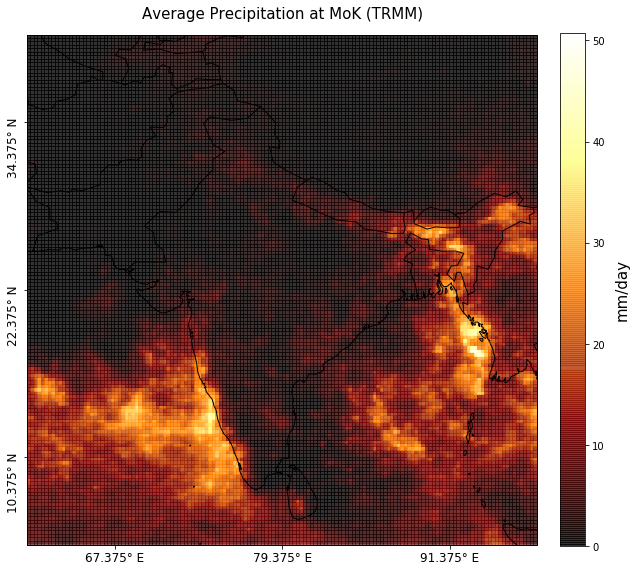
\includegraphics[width=0.4\linewidth]{./99_appendix/img/prec_avg_onset}
  \caption{Average precipitation at MoK (TRMM, 1998-2017)}
  \label{fig:trmm_prec_onset}
\end{figure}

We found that, in this case, the models learned a way to get close to the real outcomes without learning anything particularly useful about the patterns in the input data: all the outcomes of the validation and test sets were simply predicted to be the mean value of the outcomes in the training set. There could be several explanations for this behavior, of which most suggest that something is off with the input data. It might be that the sparsity of the TRMM dataset (as visualized in \cref{fig:trmm_prec_onset}) and its many places without any rainfall prevent the neural network from learning any useful patterns. Alternatively, it could be that we are trying to find patterns in the input data that don't exist in the way we would have imagined (i.e., that we are trying to fit a model to noise).

\subsubsection{E1: Convolutional models using ERA-Interim}
\label{sst:nn_e1}
The overall results from T1 up to T4 suggested that the TRMM dataset on its own might not be well suited for the prediction task at hand. An obvious way of improvement was to use another dataset for the prediction tasks, namely the ERA-Interim reanalysis dataset.

Compared to the TRMM dataset, the ERA-Interim dataset brings with it several advantages relevant to our task. Firstly, much more data is available (dating back to 1979 instead of 1998), which can improve the performance of deep neural networks significantly (even though the number of total examples is still comparatively small). Secondly, there are many more features (of which some could prove to be better predictors than solely the amount of daily rainfall). Furthermore, the dataset had already been used for onset prediction tasks in \citep{Stolbova.2015}.

A disadvantage of using the ERA-Interim dataset might be that its spatial resolution is much lower than the one of the TRMM dataset (0.75\degree x 0.75\degree compared to 0.25\degree x 0.25\degree). When training with the ERA-Interim dataset, the input matrices in the sequence would thus be much smaller in the spatial dimensions (latitude and longitude), providing the models with less detailed data to train on. However, many more ERA-Interim features could be added as channels to the model inputs, giving the models the possibility to learn more complex patterns and relationships. The lower resolution of the ERA-Interim dataset further means that each input matrix is up to 9 times smaller than with TRMM, leading to lower overall computational effort and hardware requirements (i.e., memory capacity).

\paragraph{Data preprocessing}
\label{ssst:nn_e1_data}
This first iteration of the ERA-based model (E1) made use of only two features from ERA-Interim: temperature and relative humidity each at a 1000hPa pressure level. \citet{Stolbova.2015} found this combination of features to be a reliable predictor of the monsoon onset date. While this finding should also apply to our problem, the approach used was based on statistical time-series analysis and prediction and as such might not directly transfer to the training of our neural network models.

To feed temperature and relative humidity to the model simultaneously, the features needed to be stacked in a single coordinate grid. Each grid cell would thus contain multiple channels (i.e., features, same as the RGB channels in images) and be represented as a 3D-tensor (i.e., a "3D matrix"). Combining grids to a sequence yielded a sequence of 3D-tensors (a 4D-tensor) that could then be used as input for the neural network models.

\paragraph{Modeling}
\label{ssst:nn_e1_modeling}
Incorporating these findings into a new model structure, we extended the convolutional and regularized T4 model to be able to learn from a sequence of 3D-tensors. The convolutional layers would then process these inputs just like they would process an RGB image with its three channels. The architecture for this is shown in \cref{lst:model_e1}.

\begin{listing}[h!]
  \begin{minted}[linenos,
    numbersep=5pt,
    gobble=4,
    frame=lines,
    framesep=2mm]{python}

    # start building a sequential model
    model = Sequential()

    # add a ConvLSTM2D layer
    model.add(
      ConvLSTM2D(
        filters=16,
        kernel_size=(7, 7),
        activation='tanh',
        recurrent_activation='hard_sigmoid',
        kernel_regularizer=regularizers.l2(0.02),
        recurrent_regularizer=regularizers.l2(0.02)))

    model.add(MaxPooling3D(pool_size=(1, 2, 2)))
    model.add(BatchNormalization())
    model.add(Dropout(0.6))

    # ... repeat with 5x5/8 and 3x3/4

    # flatten to make data digestible for dense layers
    model.add(Flatten())
    model.add(BatchNormalization())

    # add a new dense layer
    model.add(Dense(1024, activation='relu', kernel_regularizer=regularizers.l2(0.02)))
    model.add(BatchNormalization())
    model.add(Dropout(0.6))

    # ... repeat with 512 and 256 nodes

    # final dense layer for numerical prediction
    model.add(Dense(1))

    # compile the model
    model.compile(
      loss='mean_squared_error',
      optimizer=RMSprop(lr=0.01),
      metrics=['mean_squared_error', 'mean_absolute_error'])

  \end{minted}
  \caption{Simplified Python pseudocode for an exemplary E1 model (default configuration).}
  \label{lst:model_e1}
\end{listing}

\paragraph{Preliminary results}
\label{ssst:nn_e1_results}
Running experiments for the E1 model yielded results that displayed similar patterns to the TRMM-based models evaluated before: the models were learning up to a certain point and plateaued at unsatisfactory levels of loss and validation loss. They still seemed to get stuck during the learning process.

As experiments for entirely different datasets (TRMM and ERA) and many hyperparameter tunings for each showed similarly unsatisfactory patterns, it was probable that something was off with the data being fed into the model. Further research showed that the distribution of onset dates used seemed to show some irregularities that had not been regarded as irregular before: many onset dates were set in the first half of May (as early as on the 12th of May), which is highly improbable for typical ISM onsets\footnote{This was brought to light during consultation with V. Stolbova.}. These onset dates might, for example, have been caused by bogus monsoon onsets that were not registered as such at the time.

The labels of the training, validation and test examples were all calculated using the skewed onset dataset. The early outliers in the dataset forced us to predict even earlier, which is why predictions up to this point were always made on the 11th of May, and why the sequences were restricted to the 72 days in between 01.03-11.05 of each year.

\subsubsection{E2, E3 \& T5: Convolutional models with objective onset dates}
\label{sst:nn_e2t5}
After further analysis of onset distributions for different onset datasets, the objective definition of monsoon onset proposed by \citet{Singh.2009} seemed to be the most adequate for our training. The distribution seemed to be much less skewed overall, with more similarities to a uniform distribution than to a Gaussian normal distribution, at least when data was restricted to the relevant area between 1979-2017 (see \cref{apx:onset_dates} for the full analysis). Notice that we found out only during the final evaluation of the E4 models that the IMD onsets calculated by \citet{Singh.2009} work even better.

While it might be counterintuitive that the ISM onset would not follow a normal distribution (as many natural processes do), a more balanced distribution of labels can improve the performance of machine learning models. Many models work better if input data is preprocessed with stratification methods (i.e., classes are rebalanced), as the model might otherwise tend to predict the label that occurs most often in the training set.

Building on these findings, we then created the E2, E3 and T5 model versions, i.e., new models for both ERA-Interim and TRMM (as well as a combination of them) that were primarily a repetition of the best previous experiments with updated labels for the new onset dates.

\paragraph{Data preprocessing}
\label{ssst:nn_e2t5_data}
Due to the new distribution of onset dates, the prediction date was newly set on the 22nd of May, increasing the available sequence length by 11 days (up to 83 days). The preprocessing otherwise didn't change much, as the TRMM dataset could simply be regarded as a one-channel version of the stacked ERA-Interim features.

\paragraph{Modeling}
\label{ssst:nn_e2t5_modeling}
The models were not much changed either, as they were already flexible enough to accept arbitrary sequence lengths and an arbitrary number of stacked features (channels). The main changes were mostly refactorings and optimizations in the order of layers. As such, we don't explicitly show the source for these kinds of models.

\paragraph{Preliminary results}
\label{ssst:nn_e2t5_results}
Running the experiments for E2 and T5 yielded much better final losses. The validation loss could get as close as 2.5 days (TRMM) and 4.7 days (ERA) of mean-absolute error, which would suggest that T5 could predict the monsoon onset on the 22nd of May and do so with an accuracy of +- 2.5 days, which would have been a good result.

However, close examination of the actual predictions of the model was not as reassuring, as the model still seemed to predict only one single number for any validation or test example that was fed into the model. Furthermore, a combination of the TRMM and ERA dataset by stacking the three features yielded comparable results: the model again seemed to resort to predicting the mean of onsets based on the TRMM dataset. Additionally, stacking the TRMM and the ERA-Interim dataset necessitated that we excluded years before 1998 from the ERA-Interim dataset, causing a hefty loss of available training data.

\subsubsection{The development of the E4-models}
\label{sst:nn_e4}
Following the bad generalization capabilities of all models up to their latest versions, an improvement to the overall training approach was sought. Up to versions E3 and T5, the dates of prediction were always fixed to a single date during the pre-monsoon period (22nd of May). This meant that for each year of data, only a single sequence could be extracted and used as a training example.

The patterns during the pre-monsoon period might not be conclusive enough to allow a model to predict future onsets reliably. Some patterns might be closely tied to a temporal distance to the monsoon onset, i.e., some event might always happen approximately two weeks before onset. This would have been captured by the model at different steps in the sequence, which could, in turn, have been suitable for prediction. On the other hand, the model might have missed many of these events because the data was cut off at a fixed prediction date, possibly multiple weeks before the real onset date.

To allow a model to capture all the events leading up to the onset of each respective year, the approach to training the model thus needed to be changed. Firstly, the model needed to be fed sequences with equal distances to the respective real onset date. For example, with an onset on the 10th of June, the sequence to be fed to the model could include data from the 9th of May to the 9th of June. Repeating this for each year in the training set while keeping a one-day distance to the real onset date and the length of the sequences fixed, the model should learn to predict that the onset will take place in exactly one day.

This would not be that useful by itself, as the model would then only be able to predict the onset one day in advance. However, this approach to training allows feeding the model multiple sequences per year, each with a different offset to the onset date and a correspondingly different label. The amount of available examples is as such greatly increased: generating three such sequences per year would triple the overall number of examples available for training. Furthermore, the prediction capabilities of the model could then be evaluated separately for each offset, yielding results on how well the model can predict one day in advance, one week in advance or even multiple weeks in advance.

The detailed architecture and evaluation of this final model architecture have already been described in depth in previous sections (\cref{e4}). Having described all the models that we used during the creation of this work, we now conclude this chapter in the next section, and our work in the section after that.

\section{Conclusion}
[TODO: TBD]
